\documentclass[diss.tex]{subfiles}

\begin{document}
\chapter{Implementation}
\label{chap:implementation}
\section{Implementation tools}
Since I was building a distributed system, it was useful to find a way to simulate multiple replicas locally on one machine. I therefore used Docker\footnote{https://www.docker.com/} to run instances of an application in a \textit{container}, with the host's X11 socket being shared with each \textit{container}, so that I could interact with each instance's GUI when it was built. This allowed for some basic bug finding in the library and application and so helped me to write unit tests to cover those cases.

I also made use of the JetBrains PyCharm IDE\footnote{https://www.jetbrains.com/pycharm/} to easily manage large numbers of files and find and replace across them. Its feature-rich debugger was also very helpful in finding sources of errors in the code. 

\section{CRDT Ordered List Library}
I began the project by creating classes for common things I would be representing in the project, making use of Python's object oriented features. As shown in Figure \ref{fig:ops}, I decided to differentiate between operations that originated from this replica (\textit{local}) and from another replica over some network (\textit{remote}). Thus, performing a \textit{local} operation executes both \textsc{atSource} and \textsc{downstream} from the updating functions, whilst performing a \textit{remote} operation executes only \textsc{downstream}. Additionally, performing a local operation uses the \textit{cursor}, state kept locally to each replica, which is an identifier of a vertex $v_C$. Performing an \texttt{OpAddRightLocal($a$)} will insert the character $a$ immediately to the right of $v_C$ before updating the cursor to point to this new vertex. Performing an \texttt{OpDeleteLocal()} deletes $v_C$ and then sets the cursor to be the identifier of its predecessor.


% DIAGRAM OPERATION HIERARCHY
\begin{figure}[H]
\begin{tikzpicture}[
  every node/.style = {shape=rectangle, rounded corners, rectangle split,rectangle split parts=2,
    draw, align=center, font=\small,
    },
    level 1/.style={sibling distance=16em},
    level 2/.style={sibling distance=12em}]]
  \node {\texttt{Op}}
  	child { node {\texttt{LocalOp}}
      child { node [fill=lightgray, ] {\texttt{OpAddRightLocal} \nodepart{second} $atom: T$ }} 
      child { node [fill=lightgray] {\texttt{OpDeleteLocal}} }
      }
    child [level distance=6em] { node {\texttt{RemoteOp} \nodepart{second} $opID :$ \texttt{ClockID}} 
		child { node [fill=lightgray] {\texttt{OpAddRightRemote}\nodepart{second} $v_l : vertex,~v: vertex$ } }
		child { node [fill=lightgray] {\texttt{OpDeleteRemote} \nodepart{second} $v: vertex$} }    
    };
\end{tikzpicture}
\caption{Class hierarchy for the supported CRDT operations. All are subtypes of \texttt{Op}, which represents any kind of operation. Shaded classes are concrete. Type $T$ must be representable as a string.}
\label{fig:ops}
\end{figure}
%
%
%
%
%
%
%
%
I also created an \texttt{Identifier} abstract class to represent the identifiers in the vertices. Since RGA and LSEQ use different kinds of identifiers, they have different implementations of this (\texttt{ClockID} and \texttt{PathID} respectively).

I wanted to be able to perform operations on and get representations of the CRDT without knowing its underlying representation (the concept of encapsulation in OOP), so created another abstract class \texttt{BaseOrderedList} from which my implementations of RGA and LSEQ (\texttt{LLOrderedList} and \texttt{LSEQOrderedList} respectively) inherit. 

Finally, the class \texttt{ListCRDT} was created to take a \texttt{BaseOrderedList}, be given \texttt{Op} objects to perform on it, and be queried for its representation. Performing a \textit{local} operation returns the equivalent \textit{remote} operation that should be performed at other replicas. For example, performing a \texttt{OpDeleteLocal()} with the cursor at $v_C$ returns a \texttt{OpDeleteRemote($v_C$)}, which will have the same effect on the representation of the list at other replicas.

A design decision was made not to support nested CRDTs (each atom is itself a CRDT) for simplicity, as moving cursors around them quickly becomes non-trivial. So, as long as an atom can be represented as a string (which all python objects can through the method \textsc{str}), it is valid, and the representation of that atom is \textsc{str}($atom$).

Here is example Python code for how \texttt{ListCRDT} performs a \texttt{OpAddRightLocal} operation. It maintains a \texttt{ClockID} object \textit{clock}, which has a timestamp, the \textit{rid}, and an \textsc{increment} function to increment the timestamp. The \textit{clock} holds the timestamp and \textit{rid} of the last locally inserted vertex, so is incremented before inserting a new one. This is the implementation of the \textsc{now} function as described in the previous chapter. \textit{self.olist} is a reference to a \texttt{BaseOrderedList} object.

\begin{figure}[H]
\begin{lstlisting}
def addRight(local_add_op):
	# the atom to insert
	atom = local_add_op.atom
	
	# generate fresh timestamp
	self.clock.increment()

	# returns the new vertex and its predecessor in the list
	left_vertex, vertex_added = 
		self.olist.addRight(self.cursor, (atom, self.clock))

	# update the cursor so that a further insert will insert just after the new vertex
	self.cursor = vertex_added.identifier

	return OpAddRightRemote(left_vertex, vertex_added)
\end{lstlisting}
\caption{How \texttt{ListCRDT} performs an \texttt{OpAddRightLocal}}
\label{fig:listcrdtaddright}
\end{figure}

\subsection{Na{\"i}ve Implementation - \texttt{ArrOrderedList}}
My first attempt at an implementation of \texttt{BaseOrderedList} for RGA was \text{ArrOrderedList}, which uses Python's builtin \texttt{list} (an array) to store the vertices. In a standard array, the time taken to find an element is linear in its size, so to improve this I store a Python \texttt{dict} (hash table) mapping a vertex's identifier to the position in the array, giving a constant time lookup.  However, inserting into the array takes time linear in its size, giving \textsc{AddRight} a cost of $O(n)$ for $n$ the current number of vertices stored. This wasn't ideal, so a different implementation was used in the end (below), but this implementation was kept for comparison. 

\subsection{RGA - \texttt{LLOrderedList}}
Since the data structure the CRDTs represent is an ordered list, it makes sense to hold the vertices as a linked list, as insertion and deletion on arbitrary positions in the list are independent of its size (unlike Python's builtin \texttt{list}). There is then a \texttt{dict} to lookup the node of each vertex in the linked list in constant time. Hence, both the \textsc{AddRight} and \textsc{Delete} functions can be performed on the list in constant ($O(1)$) time in the average case, if the hash table is sufficiently balanced (slots are filled evenly).

\subsection{LSEQ - \texttt{LSEQOrderedList}}

For LSEQ, it is possible to know where to insert a vertex purely based on its position. Therefore, the downstream phase of \textsc{AddRight($v_l$, $v$)} can be simplified to \textsc{Add($v$)} (this will come in useful when implementing \textit{undo} in section \ref{sec:undo}). However, this means a data structure that can support this is needed. So, the requirements for such a data structure are:
\begin{itemize}
\item Fast finding of next and previous elements
\item Fast lookup of an element given its identifier
\item Fast lookup of the element with the largest identifier smaller than a given identifier (the in-order predecessor)
\end{itemize}
The linked list approach used for RGA would satisfy the first two criteria, but would require a linear scan for the third. The tree-like nature of the positions in LSEQ suggests a tree-like data structure, and indeed I found the \texttt{SortedList}\footnote{\url{http://www.grantjenks.com/docs/sortedcontainers/sortedlist.html}} from the \texttt{SortedContainers} Library. It offers roughly logarithmic time insertion and deletion (verified in the Evaluation chapter), and has a method \textsc{bisect\_left} for finding the index of the smallest element greater than a given one (meaning one less than this index points to the largest element smaller than the given one when the given one is not in the list).

While implementing LSEQ, I came across a further improvement to the scheme \cite{hlseq}. The motivation was that replicas would all be choosing different random bits for the \textsc{alloc} function, so it would be better if they could collude. The h-LSEQ scheme achieves this by having a pseudorandom sequence generated by a seed shared by all replicas. Thus, each replica uses LSEQ, but all replicas have the same strategies.

%%%%%%%%%%%%%%%%%%%%%%%%%     UNDO       %%%%%%%%%%%%%%%%%%%%%%%%%

\subsection{Undo/Redo}\label{sec:undo}
Having seen a paper implementing a global undo for a CRDT-based editor \cite{logootundo} (based on theory from \cite{undoatanytime}), I decided to also implement an undo function, but only locally. That is, a replica can undo and redo the operations it originated, but no others. Being able to undo all replicas' operations seemed messy and frustrating from a user's perspective. For example, one user accidentally deletes a character, then just as they are about to press `undo', their collaborator inserts a character. Pressing undo would delete the collaborators inserted character (to their annoyance) and the user's deletion wouldn't get undone (to the user's annoyance). 

After an operation is performed, it is stored in a list specific to its originating replica (see section \ref{sec:helper} for details). As shown in Figure \ref{fig:undostorage}, the operations originating at this replica can be undone by popping them from $opStore$ (for this replica), performing their inverse and pushing that to a special stack of undone operations. To redo, pop from $undoStack$, perform the inverse operation, and push that to $opStore$. To avoid a branching history, when a new operation originating at this replica is performed (one that has not been undone or redone), $undoStack$ is emptied.

\begin{figure}[H]
\centering
\begin{tikzpicture}[trim left = (elsewhere), >={Latex[scale=1.5]}]
\path 
(3cm, 0) pic {stack=1}
(-3cm, 0) pic {stack=4};
\node  at (-3cm, -15pt){$opStore[rid]$};
\node  at (3cm, -15pt){$undoStack$};
\node (opstore) at (-3cm, 3cm) {};
\node (undostack) at (3cm, 3cm) {};
\node (elsewhere) at (-7cm, 3cm) {};
\draw[->, out=45, in=135] (elsewhere) to node[above] {\begin{tabular}{c} perform local \\ (+ clear $undoStack$) \end{tabular}} (opstore);
\draw[<->, in=30, out=150] (undostack) to node[below] {redo} node[above] {undo} (opstore) ;
\end{tikzpicture}
\caption{How operations are undone and redone at replica with id $rid$}
\label{fig:undostorage}
\end{figure}

\begin{figure}[H]
\begin{tikzpicture}[
  every node/.style = {shape=rectangle, rounded corners, rectangle split,rectangle split parts=2,
    draw, align=center, font=\small,
    },
    level 1/.style={sibling distance=16em},
    level 2/.style={sibling distance=12em}]]
  \node {\texttt{LocalOp}}
  	child { node [rectangle split parts=1] {\texttt{...}}}
    child { node [fill=lightgray] {\texttt{OpUndo} \nodepart{second} $op:RemoteOp$}}
    child { node [fill=lightgray] {\texttt{OpRedo} \nodepart{second} $op:RemoteOp$}};
\end{tikzpicture}
\caption{How OpUndo and OpRedo fit into the operation hierarchy}
\label{fig:undoops}
\end{figure}

With only the vertex to be deleted stored in \texttt{OpDeleteRemote}, it is not possible to fully invert it to an \texttt{OpAddRightRemote} as the left vertex ($v_l$) is unknown. However, the LSEQ scheme doesn't necessarily require a left vertex, so we may leave out the left vertex property of the \texttt{OpAddRightRemote} and just consider a one argument constructor taking the vertex to be inserted. So, for brevity here I will refer to \texttt{OpAddRightRemote}($v$) as \texttt{Add}($v$) and \texttt{OpDeleteRemote} as \texttt{Delete}($v$). This means undo isn't supported when using RGA. 

When the application initiates an undo (respectively redo), an \texttt{OpUndo} (\texttt{OpRedo}) operation is created with the most recent operation from $opStore$ of this replica (resp. $undoStack$) as a parameter to its constructor. The \texttt{ListCRDT} object has logic (a function \textsc{undo}) for taking an operation and performing the inverse of it on the \texttt{BaseOrderedList} object.

\begin{algorithm}[H]
\caption{How \textsc{inverse} inverts operations}
\begin{algorithmic}[1]
\Function{inverse}{\texttt{Add}($v$)}
\State \Return \texttt{Delete}($v$)

\EndFunction
\end{algorithmic}

\hrule 

\begin{algorithmic}[1]
\Function{inverse}{\texttt{Delete}($v$)}

\State \Return \texttt{Add}($v$)
\EndFunction
\end{algorithmic}
\end{algorithm}

This \textsc{undo} function is the same for \texttt{OpUndo} and \texttt{OpRedo} as to redo an operation is to undo the operation which undid it. For example, imagine an $x$ is inserted into some list. Undoing this deletes it. Redoing the insertion then amounts to undoing the deletion. 


% cemetary + visibility numbers etc.
To support undo, I had to amend the logic in \texttt{LSEQOrderedList}'s code for list operations in line with \cite{logootundo}. Firstly, each vertex $v$ has an associated \textsc{count} function (returning an integer) such that the vertex appears in the document if and only if $\textsc{count}(v) = 1$. A vertex's count starts at 0 and is incremented when it is inserted, and decremented when it is deleted.

It may seem at first that we have to store this count for every vertex, but in fact only a very small number need to be stored. The \textit{cemetary} is a \texttt{dict} mapping vertex identifiers to counts only if the count is less than 0. This happens when there are concurrent deletions of the same vertex, and as soon as the count becomes 0 or 1, the entry is removed. The number of concurrent deletions present in the document is expected to be very small, so this overhead is minimal. For any other vertex, if it is present in the list data structure its count must be 1 (it appears in the representation of the list), and if not then its count is 0.



% amended add/delete pseudocode
%
\begin{algorithm}[H]
\caption{Pseudocode for the cemetary operations and the amended list operations to support undo/redo (\textsc{AddRight} is now just \textsc{Add})}
\begin{algorithmic}[1]
\Function{cemetaryGet}{$id$} \Comment lookup $id$ in the cemetary
\If{$id \in cemetary$}
\State \Return $cemetary[id]$
\Else
\State \Return $0$ \Comment return 0 if $id$ is not in the cemetary
\EndIf

\EndFunction
\end{algorithmic}

\hrule 

\begin{algorithmic}[1]
\Function{cemetarySet}{$id$, $degree$} \Comment Update the count for $id$
\If{$degree = 0$}
\State \textsc{del} $cemetary[id]$	\Comment $degree >= 0$ so doesn't need to be stored
\Else
\State $cemetary[id] \gets degree$
\EndIf
\EndFunction
\end{algorithmic}

\hrule 

\begin{algorithmic}[1]
\Function{Add-downstream}{$v$}\Comment Increment $\textsc{count}(v)$
\State $(a, id) \gets v$
\State $degree \gets \Call{cemetaryGet}{id} + 1$
\If{$degree = 1$}
\State $l \gets l \cup \{v\}$ \Comment Now $\textsc{count}(v)=1$
\Else
\State \Call{cemetarySet}{$id$, $degree$}
\EndIf



\EndFunction
\end{algorithmic}

\hrule 

\begin{algorithmic}[1]
\Require state $l = \langle ..., v_l, v, v_r, ... \rangle \vee v \notin l$
\Function{Delete-downstream}{$v$} \Comment Decrement $\textsc{count}(v)$
\State $(a, id) \gets v$
\If{$v \in l$} \Comment $\textsc{count}(v)=1$
\State $l \gets \langle ..., v_l, v_r, ... \rangle$ \Comment Remove $v$ from the list, $\textsc{count}($v$) = 0$

\Else
\State $degree \gets \Call{cemetaryGet}{id} - 1$
\State \Call{cemetarySet}{$id$, $degree$} \Comment decrement \textsc{count}($v$)
\EndIf

\EndFunction
\Ensure $v \notin l$
\end{algorithmic}
\end{algorithm}
%
%





%%%%%%%%%%%%%%%%%%%%%%%%% HELPER STRUCTURES %%%%%%%%%%%%%%%%%%%%%%%%%



\section{Application Library}\label{sec:helper}
\begin{figure}[H]
\centering
\begin{tikzpicture}[every node/.style={draw},>={Latex [scale=2]} ]
\node[draw](App) at (0,0) {\texttt{CRDTApp}};
\node[above right of = App, xshift=2.5cm, draw, yshift=1cm](OpStore) {$opStore$};
\node[below right of = App, draw, xshift=2.5cm, yshift=-1cm](ListCRDT) {\texttt{ListCRDT}};
\path 
(-5cm,0.5cm) pic[local bounding box=Queue] {queue=5};
\node [draw=none] at (-3.5cm, -1cm){$opQueue$};

\node[above left = 1cm of Queue, yshift=1cm](Network) {\texttt{CRDTNetworkClient}};
\node[below left = 1cm of Queue, yshift=-1cm](UI) {\texttt{CRDTLocalClient}};

\node[below = 2cm of Queue](heldback) {$heldBackOps$};


\node[cloud, cloud ignores aspect, cloud puffs=13.5, minimum width=1cm,
minimum height=0.5cm, above of =Network, yshift=1cm](Cloud) {other replicas};

\draw[->] [in=-90, out=east]([yshift=0.1cm]App.east) to node[near end, draw=none, right, xshift=0.2cm] {2. store} (OpStore.south);
\draw[->][in=90, out=east] ([yshift=-0.1cm]App.east) to node[near end, draw=none, right, xshift=0.2cm] {1. perform} (ListCRDT.north);

\draw[->] (Queue) -- (App);

\draw[->] [out=north, in=0] (App.north) to node[draw=none, near end, above] {3. send} (Network.east);

\draw[->] [out=south, in=west] (Network.south) to ([xshift=1cm]Queue.west);
\draw[->] [out=north, in=west] (UI.north) to node[draw=none, left, pos=0.3] {KeyEvent}([xshift=1cm]Queue.west);

\draw[->] [out=south, in=east] (App.south) to node[midway, draw=none, right] {4. recover} (heldback.east);
\draw[->] [out=north, in=south](heldback.north) to (Queue.-20);



\draw[<->] (Network.north) to (Cloud.south);

\end{tikzpicture}
\caption{The layout of the application; arrows indicate the flow of operations. The numbers indicate the order in which \texttt{CRDTApp} does these actions}
\label{fig:app}
\end{figure}
To build an application that uses the CRDT library required a few extra data structures to move around and store operations. 
The first problem to be dealt with is that operations will arrive asynchronously from both the network and any local GUI the application is connected to. It therefore makes sense to use the \textit{producer-consumer} paradigm and have a queue of operations that the network and GUI feed into, and a separate thread pulls out of to perform them (two producers and one consumer).

%%      op queue       %%

To that end, \texttt{OperationQueue} is a class I built that wraps around Python's \texttt{Queue} class, a thread-safe, double-ended queue. It adds a \texttt{Semaphore} (from Python's \texttt{threading} module) for condition synchronisation, such that the consuming thread can, on seeing an empty queue, block until something is available instead of busy waiting. When a producing thread adds to the queue, it increments the semaphore, and a consumer decrements it on receiving. If the semaphore is 0 a decrement will block until there is an increment. The application's instance of the \texttt{OperationQueue} will be referred to just as $opQueue$.

I then created a class \texttt{OperationStore} which just has a \texttt{dict} of \texttt{list}s (Python builtins) and exposes operations on it.

\begin{algorithm}[H]
\caption*{Methods supported by \texttt{OperationStore}}
\begin{algorithmic}[1]
\Function{addOp}{$key$, $op$} \Comment{stores $op$ in the list indexed by $key$}
\EndFunction
\Function{getOpsForKey}{$key$} \Comment{returns the list indexed by $key$}
\EndFunction
\end{algorithmic}
\end{algorithm}

Since it was the case that multiple threads may be accessing instances of this simultaneously, and Python has no \textit{synchronized} primitive like Java, I needed some way of having thread-safe access to the structure beyond Python's Global Interpreter Lock (mainly for iterating over parts of it safely). This was achieved with a \textit{synchronized} decorator\footnote{https://github.com/openstack/deb-python-wrapt} to decorate the necessary functions such that only one thread can access the object they are tied to at a time.

Recall that operation-based CRDTs traditionally require that if $A$ \textit{happens-before} $B$, $A$ should be delivered (and hence here performed) before $B$. To provide this, each operation sent (any \texttt{RemoteOp}s) has an $opID$ (instance of \texttt{ClockID}), a pair of a timestamp and $rid$ showing the operation's source replica. Since a causal order on events implies the order of their timestamps, but not the other way round, from two $opID$s we can only infer one operation \textit{happens-before} the other from their timestamps if their $rid$s are the same. Such Lamport clocks \cite{lamportshappensbefore} can be extended by using a vector of such clocks (one per replica) meaning from comparing vector clocks, causal order can be inferred.

In this application, I decided that keeping strict causal order denies some orderings that actually work, so kept to Lamport clocks and a weaker-than-causal order to boost performance. The proof that such an ordering is appropriate is in the Appendix.

As will be seen in section \ref{sec:networking}, the way operations are sent guarantees operations with the same source replica will be ordered correctly. However, there needed to be a way of dealing with ordering dependent operations from different source replicas whose order cannot be inferred from their $opID$s.

As shown in Figure \ref{fig:deliveryorder}, it may be that an operation arrives before a causal predecessor over a network. On seeing a timestamp more than one greater than the last we have seen from any replica, we don't know if we have missed one. For example, if there was also an operation 1:C, then on seeing 2:B, replica C wouldn't know if there was a 1:A coming, because it could have been 1:C that incremented B's clock. To resolve this ambiguity, I attempt to perform operations, and if they reference vertices that don't exist yet, the operations fails with a \texttt{VertexNotFound} exception, they get \textit{held back} and are performed when that vertex does exist, so the resulting order may not be causal, but respects all dependencies (defined in the Appendix).

\begin{figure}[H]
\centering
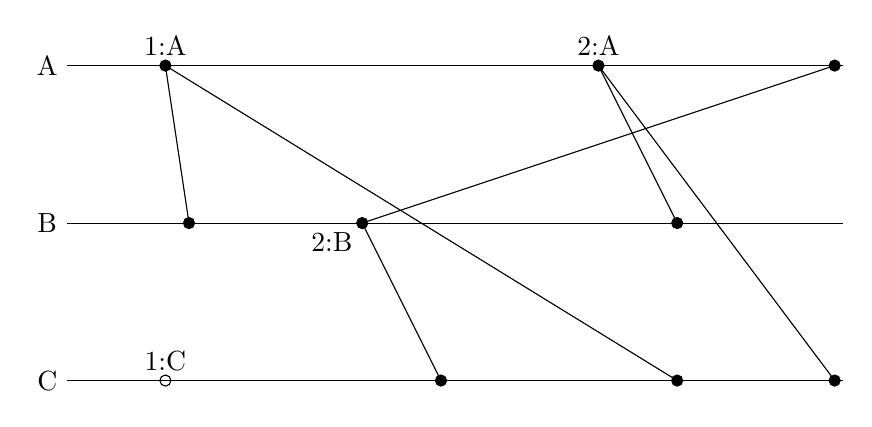
\begin{tikzpicture}
\node(A) at (-5cm, 2cm) {A};
\draw (A) -- ++ (\linewidth-\pgflinewidth-2cm, 0);
\node(B) at (-5cm, 0) {B};
\draw (B) -- ++ (\linewidth-\pgflinewidth-2cm, 0);
\node(C) at (-5cm, -2cm) {C};
\draw (C) -- ++ (\linewidth-\pgflinewidth-2cm, 0);

\draw (-3.5cm, -2cm) circle (2pt) node[above] {1:C};

\filldraw (-3.5cm, 2cm) circle (2pt) node[above] {1:A} -- (-3.2cm, 0) circle (2pt);
\filldraw (-3.5cm, 2cm) -- (3cm, -2cm) circle (2pt);

\filldraw (-1cm, 0) circle (2pt) node[below left] {2:B} -- (5, 2cm) circle (2pt);
\filldraw (-1cm, 0) -- (0cm, -2cm) circle (2pt);

\filldraw (2cm, 2cm) circle (2pt) node[above] {2:A} -- (3cm, 0) circle (2pt);
\filldraw (2cm, 2cm) -- (5cm, -2cm) circle (2pt);
\end{tikzpicture}
\caption{An example sending of operations with $opID$s 1:A, 2:A and 2:B. The latter arrives at C before its causal predecessor 1:A.}
\label{fig:deliveryorder}
\end{figure}

To achieve this, there is an implementation of \texttt{OperationStore} called $heldBackOps$, on which \textsc{addOp}($ vertexID$,$op$) is called for when the operation $op$ fails which references a vertex with identifier $vertexID$ (if \texttt{OpAddRightRemote} this is the identifier of the left vertex $v_l$ and for a \texttt{OpDeleteRemote} is the identifier of the vertex to be deleted). For example, in RGA, an \textsc{AddRight} would fail if the left vertex didn't exist, and a delete would fail if the vertex to be deleted didn't exist. Now, after performing an operation with identifier $opID$, we call \textsc{getOpsForKey}($opID$) on $heldBackOps$ and add any operations in the resulting list to the front of $opQueue$ (called the $recovery$ phase). This works because the $opID$ of an \texttt{OpAddRightRemote} has the same timestamp and $rid$ as the inserted vertex. So, on inserting the vertex, we free and perform any operations waiting on that vertex to exist.


Another structure needed is a way to keep track of which of whose operations a replica has performed, so that it may share operations with new replicas that come online to collaborate. Let this be known as $opStore$. This is an implementation of \texttt{OperationStore}, keeping lists of performed operations indexed in the \texttt{dict} by source replica. Operations in a list are kept in the order they were performed at this replica. So, each list will be ordered by the timestamps of the $opID$s as two operations with the same source replica cannot be concurrent. 

As such, the \texttt{CRDTApp} has a thread which loops continuously over the following sequence:

\begin{itemize}
\item Pop from $opQueue$
\item Perform the popped operation
\item Store the operation that results from performing
\item Send the operation to any other replicas connected
\item Do $recovery$: check if any operations were waiting on this one to complete
\end{itemize}

Finally, in order to know who to send operations to (ie who you are currently collaborating with), there is a structure \texttt{ConnectedPeers} which wraps around Python's \texttt{dict} providing friendly methods for storing peer information and a thread-safe way to iterate over it. Applications each have an instance of this known as $connectedPeers$.
%
%
%
%
%
%

\subsection{GUI Application}
The first extension to the project I implemented was a simple graphical user interface (GUI) to allow quick identification of obvious errors in my code (helped even more by the use of Docker containers) to make a complete, runnable application. This was achieved with the use of Tkinter\footnote{https://wiki.python.org/moin/TkInter}, a Python interface to the Tk toolkit. Tk has a hierarchy of \textit{widgets}, beginning with the \textit{root}, which represent objects on the screen, where each child object is contained within its parent. Keyboard and mouse events are handled by a system of callbacks. A function may be bound to a specific event such that when that event occurs the function is called with the event information passed as a parameter.

With that in mind, I created a function to, given a keycode of a printable character, add a new \texttt{AddRightLocal} operation inserting that character to $opQueue$.  If the key was backspace, a \texttt{DeleteLocal} is added. This was bound to the \textit{KeyDown} event so the relevant operations are performed when keys are pressed. If the Left (resp. Right) Arrow Key is pressed, code is executed which calls \textsc{shiftCursorLeft(Right)} in ListCRDT. This sets the cursor to the next(resp. previous) non-deleted vertex in the list after the current cursor. A reference to the latter function is passed to the object that contains the GUI code, \texttt{CRDTLocalClient}. These arrow keys could therefore easily be configured to traverse the document in some other way than just horizontally by one character. The keys to enact an undo or redo work by the same principle.

A Text widget from Tkinter is used to hold the CRDT's representation. This captures keyboard events and sends them to the aforementioned bound functions. It has a method for setting the position of its insertion cursor as well, which takes a line and column index. I decided to restrict the editor to only single-line text for ease of moving the cursor around (the only valid moves are to the next or previous vertices that aren't deleted) and so pressing \textit{return} does not trigger an event as it is not a printable character.

The GUI needs to be updated every time an operation is performed, as all operations have some effect on the representation of the CRDT. To do this, the list of vertices is iterated over and for each vertex $(a,id)$, $\textsc{str}(a)$ is appended to the output (if the vertex isn't deleted). Also, when the identifier held in the \textit{cursor} is encountered, the number of atoms output so far determines the column number that the cursor should appear in the final output. This is needed for specifying the column index when the insertion cursor in the Text widget is set.




%%%%%%%%%%%%%%%%%%%%%%%%% NETWORKING %%%%%%%%%%%%%%%%%%%%%%%%%



\section{Networking}\label{sec:networking}
To exchange operations with each other, replicas need to communicate over some network. I chose TCP/IP as the communication mechanism to allow potentially global collaboration. TCP allows for reliable, inorder delivery of data, which specifically means operations from the same replica will be delivered in the order they were sent, a required property for op-based CRDTs. 

To implement such a mechanism, I used Python's builtin \texttt{socket} library to create sockets which can be read from and written to. One socket listens for connections (the server socket) whilst the other actively connects to a listening socket (the client socket) and hence a channel is created between them. However, TCP is a stream-oriented protocol, and I needed some way to delimit separate operations.

Firstly, operations are sent by sending the actual \texttt{Op} objects. To serialize such objects into a format that can be sent, the \texttt{pickle} library\footnote{https://docs.python.org/3/library/pickle.html} is used. The pickled data is sent prefixed by a 4 byte representation of its length. In this way, a receiver knows to first read 4 bytes from the stream (= $length$), then read a further $length$ bytes to get the actual data (a technique called framing). It then unpickles this to get the \texttt{Op} object. The \textsc{recv} function on the socket object to read from it takes a maximum number of bytes you wish to receive, and returns the actual number read. As there is no guarantee that you will get the number of bytes you were expecting all at once, I repeatedly call this method until $length$ bytes of data are actually received.

In order to support pickling/unpickling, a Python object merely has to override the methods \textsc{\_\kern-.14ex\_getstate\_\kern-.14ex\_} (for pickling) and \textsc{\_\kern-.14ex\_setstate\_\kern-.14ex\_} (unpickling). In the former one must return a \texttt{dict} with values of the object's properties necessary to recover the object, and in the latter the properties are set with values from this \texttt{dict}.

As my project supports offline editing, when a replica comes online having performed operations offline, it is necessary to both share those operations with other replicas and receive any new operations from them. The set of operations needed by replica $r_k$ is $$o = \bigcup_{i\neq k} \left\{ops_{r_i}\right\} - ops_{r_k}$$ where $ops_{r_k}$ are the operations $r_k$ has either in $opStore$, $opQueue$ or is currently performing. Any connections the replica makes are in different threads, so that requests for new operations to each replica are pipelined (all requests may be sent before even one response is received). This decision was made over waiting for each response to arrive as the waiting time is bounded only by the timeout of the local TCP implementation which was deemed to be too long.

To calculate $o$, each replica keeps a vector of \texttt{ClockID} objects (the vector clock) for each replica that it has seen an operation originating from. This is updated when $opQueue$ receives a new operation. Each object's timestamp is the highest timestamp of all the operations it has seen originating from that object's replica. \texttt{OperationStore} has a method for taking a vector clock and outputting a list of operations stored that haven't been seen by that vector clock. That is, for each \texttt{ClockID} $c$ in the vector, it finds, in the list of operations it has stored for the replica corresponding to that object, any operations $o$ for which $\textsc{timestamp}(c) < \textsc{timestamp}(o)$, then combines those into one big list. Since $opStore$'s lists are kept sorted, one can use a variant of the binary search algorithm to find the smallest timestamp in the list greater than $c$'s, then return that element and all subsequent ones in the list as the result. For example, given the vector clock $5$:A $|$ $4$:B and the lists [$1$:A, $2$:A, $4$:A, $6$:A, $7$:A] and [$3$:B, $5$:B], the procedure would return [$6$:A, $7$:A, $5$:B]. Importantly, this process preserves the ordering of the operations, so the operations from each replica are sent in increasing order of their timestamps. 

Finally, when sending a new operation, you iterate over a copy of $connectedPeers$'s sockets and call \texttt{socket}.\textsc{send} on each one.


%%%%     DIAGRAM OF NETWORK CLASSES    %%%%
\begin{figure}[H]
\centering
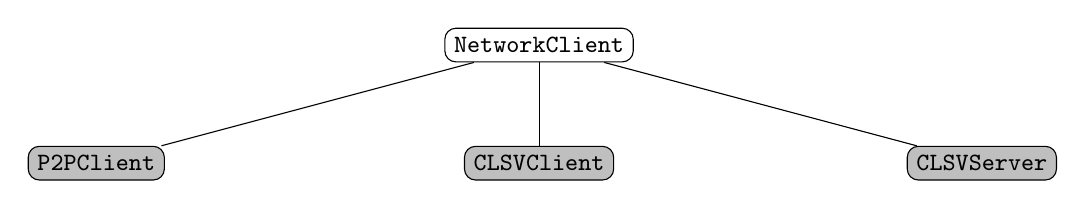
\begin{tikzpicture}[
  every node/.style = {shape=rectangle, rounded corners, draw, align=center, font=\small,
    },
    level 1/.style={sibling distance=16em},
    level 2/.style={sibling distance=12em}]]

  	\node {\texttt{NetworkClient}}
      child { node [fill=lightgray, ] {\texttt{P2PClient}}} 
      child { node [fill=lightgray] {\texttt{CLSVClient}}} 
      child { node [fill=lightgray] {\texttt{CLSVServer}}};
 
\end{tikzpicture}
\caption{The networking classes used in the application. \texttt{NetworkClient} contains common code for sending and receiving data as described above.}
\label{fig:nethier}
\end{figure}



\subsection{Client-server Architecture}

\begin{figure}[H]
\centering
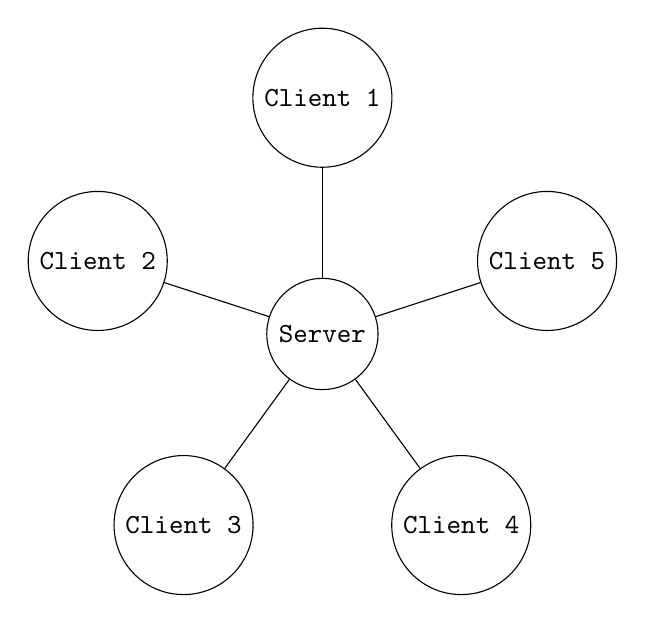
\begin{tikzpicture}[every node/.style={draw, circle}]
\def \n {5}
\node(server) at (0,0) {\texttt{Server}};
\foreach \x in {1,...,\n}{
	\node(client\x) at ({360/\n * \x + (90 - 360/\n)}:3) {\texttt{Client \x}}; 
	\draw (client\x) -- (server);
	
};
\end{tikzpicture}
\caption{The standard client-server architecture with 5 clients}
\label{fig:clsv}
\end{figure}

The first network architecture I implemented was one where there is a central server which all replicas connect to (it is not itself a replica). The server simply relays operations between replicas and stores them locally. Thus, any new replica (one that just connected and needs to know about other replicas' states) only needs to send its vector clock to the server rather than all replicas separately. So, the server keeps an instance of \texttt{ConnectedPeers} and listens to all connected clients for new operations. On receiving an operation, it stores it locally and sends it over all sockets in the \texttt{ConnectedPeers} instance. 



\begin{figure}[H]
\centering
\begin{tikzpicture}[>={Latex}]
\def \a {-3}
\def \b {3}
\def \i {-0.8}
\newcounter{seq}
\setcounter{seq}{2}
    \node[draw](A) at (\a,0) {Client (C)};
    \node[draw](B) at (\b,0) {Server (S)};
    
    %
    %
    %
    %
    %
    
    \draw[->] (\a, \value{seq}*\i) -- node[above]{optional: Diffie-Hellman}(\b, \value{seq}*\i);
    \addtocounter{seq}{1};
    \draw[<-] (\a, \value{seq}*\i) -- node[above]{optional: Diffie-Hellman}(\b, \value{seq}*\i);
    \addtocounter{seq}{2};
    
    
    \draw[->] (\a, \value{seq}*\i) -- node[above]{vector clock C}(\b, \value{seq}*\i);
    \addtocounter{seq}{1};
    \draw[<-] (\a, \value{seq}*\i) -- node[above]{vector clock S}(\b, \value{seq}*\i);
    \addtocounter{seq}{2};
    
    
    \draw[->] (\a, \value{seq}*\i) -- node[above]{$ops_C - ops_S$}(\b,\value{seq}*\i);
	\addtocounter{seq}{1};
    \draw[<-] (\a, \value{seq}*\i) -- node[above]{$ops_S - ops_C$}(\b,\value{seq}*\i);
    \addtocounter{seq}{1};
    
    \draw (A) -- ++(0,\value{seq}*\i);
    \draw (B) -- ++(0,\value{seq}*\i);
\end{tikzpicture}
\caption{The protocol for clients connecting to the server.}
\label{fig:protocolsv}
\end{figure}



\subsection{P2P Architecture}

\begin{figure}[H]
\centering
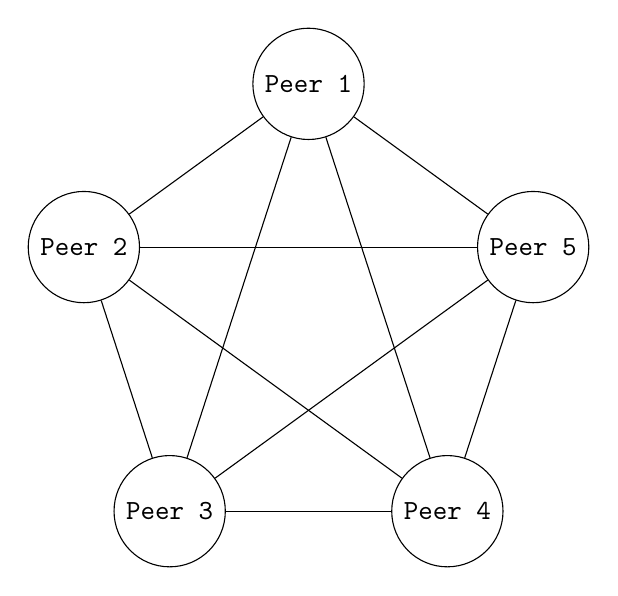
\begin{tikzpicture}[every node/.style={draw, circle}]
\def \n {5}
\foreach \x in {1,...,\n}{
\node(client\x) at ({360/\n * \x + (90 - 360/\n)}:3) {\texttt{Peer \x}}; 
\foreach \y in {1,...,\x}{
	\draw (client\x) -- (client\y);
	};
};
\end{tikzpicture}
\caption{The standard P2P architecture with 5 clients}
\label{fig:p2p}
\end{figure}

The P2P architecture (as shown in Figure \ref{fig:p2p}) consists of links from every node to every other node, making a complete graph. Therefore, it is necessary:
\begin{enumerate}
	\item For each node to know how to reach every other node
	\item For each node to listen for connections from as well as initiate connections to all other nodes
\end{enumerate}
To deal with the first requirement, a design decision was made to assume nodes who wish to collaborate know through some other channel the addresses of their collaborators. Another option considered was to have a centralized directory service which stores mappings of documents to node addresses. However, this mirrors the shortcomings of the client-server approach; namely that the directory is a single point of failure, and if compromised could reveal addresses people might want to keep private. Besides, to implement such a directory would require a new client to provide some identifier (such as a key) to the directory so they may be linked to a document. The identifier would have to be shared through some other channel anyway. Moreover, the Tor Hidden Service protocol deals with the issue of collaborators wishing their location to be hidden from the others.

For the second, it was necessary for each peer application to both have a server socket accepting incoming connections and to try and open a socket to every other peer. However, this would result in two connections for each link shown in the diagram, which is undesirable. Therefore, it is necessary to check in $connectedPeers$, and not complete a connection to an already connected peer. Unfortunately, this is still not enough, as due to the socket threads running simultaneously, both connections could make progress simultaneously, and shutting down a random one on both sides could obliterate both connections. So, asymmetry must be introduced so that the same connection is killed on both sides (ie the incoming on one side which is the outgoing on the other) . Hence, as shown in Figure \ref{fig:protocol}, peers send their name, and on detecting multiple connections to the same peer, an incoming connection is allowed only if the other peer has a lower identifier than yours.

\section{Encryption}
As the project has a theme of privacy, encrypting the channels between nodes seemed sensible. This was achieved by adding an optional Diffie-Hellman (DH) key exchange \footnote{http://mathworld.wolfram.com/Diffie-HellmanProtocol.html} to the protocol, hashing the computed shared secret to generate an AES key, then encrypting all further communications over that channel using the key and AES CCM mode\footnote{https://en.wikipedia.org/wiki/CCM\_mode}, which is Counter mode for confidentiality together with a CBC-MAC for integrity. AES-CCM is an authenticated encryption scheme that, provided it is used correctly, allows for confidentiality and integrity of all messages sent on the channel \cite{ccm}. Negotiating session keys for each channel means one can get \textit{perfect forward secrecy}, meaning compromise of nodes doesn't reveal all past keys and thereby breaking confidentiality of all past messages. This use of asymmetric encryption (in DH) to bootstrap a symmetric encryption scheme is commonly used as symmetric encryption generally is faster. However, without the use of public keys for the Diffie-Hellman step, overall this is not an authenticated encryption scheme, and is vulnerable to man-in-the-middle attacks (as described in the Evaluation chapter). This is why the authentication was used over Tor (Section \ref{sec:auth}).



\begin{figure}[H]
\centering
\begin{tikzpicture}[>={Latex}]
\def \a {-3}
\def \b {3}
\def \i {-0.8}
\setcounter{seq}{1}
    \node[draw](A) at (\a,0) {Node A};
    \node[draw](B) at (\b,0) {Node B};
    
    %
    %
    %
    %
    %
    \draw[->] (\a, \value{seq}*\i) -- node[above]{A}(\b, \value{seq}*\i);
    \addtocounter{seq}{1};
    \draw[<-] (\a, \value{seq}*\i) -- node[above]{B}(\b, \value{seq}*\i);
    \addtocounter{seq}{2};
    
    \draw[->] (\a, \value{seq}*\i) -- node[above]{optional: Diffie-Hellman}(\b, \value{seq}*\i);
    \addtocounter{seq}{1};
    \draw[<-] (\a, \value{seq}*\i) -- node[above]{optional: Diffie-Hellman}(\b, \value{seq}*\i);
    \addtocounter{seq}{2};
    
    
    \draw[->] (\a, \value{seq}*\i) -- node[above]{vector clock A}(\b, \value{seq}*\i);
    \addtocounter{seq}{1};
    \draw[<-] (\a, \value{seq}*\i) -- node[above]{vector clock B}(\b, \value{seq}*\i);
    \addtocounter{seq}{2};
    
    
    \draw[->] (\a, \value{seq}*\i) -- node[above]{$ops_A - ops_B$}(\b,\value{seq}*\i);
	\addtocounter{seq}{1};
    \draw[<-] (\a, \value{seq}*\i) -- node[above]{$ops_B - ops_A$}(\b,\value{seq}*\i);
    \addtocounter{seq}{1};
    
    \draw (A) -- ++(0,\value{seq}*\i);
    \draw (B) -- ++(0,\value{seq}*\i);
\end{tikzpicture}
\caption{The protocol for peers connecting in the P2P architecture. After exchanging identifiers, they synchronize their operations.}
\label{fig:protocol}
\end{figure}

%%%%%%%%%%%%%%%%%%%%%%%%%        TOR           %%%%%%%%%%%%%%%%%%%%%%%%%

\section{Tor}

The final extension added to the project was the use of the Tor network for communication in the P2P architecture. The idea is that each peer advertises a Hidden Service (HS), and other collaborators know its \textit{onion address} (again through some other channel), and connect to it through Tor's HS protocol \cite{torrendspec}. 

Stem, the Python library used for interacting with the Tor process, exposes a method \textsc{createEphemeralHiddenService}, which can be called to setup a HS on a machine. It can be given a private key from which the public key (and subsequently the \textit{onion address}) for the service can be derived. Users need to keep a private key for each document they work on and provide one to the application on startup. `Ephemeral' here refers to how the HS created is kept entirely in memory and does not touch the filesystem at all. 

Once the Tor process is running, to connect to a hidden service, one simply routes traffic through the local SOCKS5 proxy server the process creates. To do this, the \texttt{PySocks} library\footnote{https://github.com/Anorov/PySocks} contains a socket object with the same interface as the Python's own \texttt{socket}, except with a setting to send traffic through a proxy server.

\subsection{Client Authentication}
\label{sec:auth}

Using Stem and the \textsc{createEphemeralHiddenService} call, basic authentication can be implemented by simply passing an extra parameter. Namely, a \texttt{dict} with names as keys. The value for each of these can be \texttt{None}, in which case when the call returns and the HS is created a \texttt{dict} is returned mapping those names to randomly generated cookies. Alternatively, previously generated cookies can be specified instead of passing \texttt{None}, in which case those are returned. The cookies are somehow distributed to other peers (through some other secure channel), then they use Stem to set their Tor process's \texttt{HidServAuth} parameter to, for each other peer $c$, a pair of $c$'s onion address and the cookie for that peer. That is, telling Tor which cookie to use for each peer.

\end{document}
